%
% General structure for the revdetua class:
%
\documentclass[mirror,times]{revdetua}
%
% Valid options are:
%
%   longpaper --------- \part and \tableofcontents defined
%   shortpaper -------- \part and \tableofcontents not defined (default)
%
%   english ----------- main language is English (default)
%   portugues --------- main language is Portuguese
%
%   draft ------------- draft version
%   final ------------- final version (default)
%
%   times ------------- use times (postscript) fonts for text
%
%   mirror ------------ prints a mirror image of the paper (with dvips)
%
%   visiblelabels ----- \SL, \SN, \SP, \EL, \EN, etc. defined
%   invisiblelabels --- \SL, \SN, \SP, \EL, \EN, etc. not defined (default)
%
% Note: the final version should use the times fonts
% Note: the really final version should also use the mirror option
%
%* Packages Used

\usepackage[english]{babel}
\usepackage[utf8]{inputenc}

\usepackage{verbatim}
\usepackage{fancyvrb}

\usepackage{listings}
\usepackage{xcolor}


\usepackage{amsmath}
\usepackage{graphicx}
\usepackage{hyperref}
\usepackage{geometry}
\usepackage{float}
\usepackage{array}

%* Package settings
\hypersetup{
colorlinks  = true,
linkcolor   = black,
urlcolor    = red,
}

\newgeometry{
      top = 0.75in,
      bottom = 0.75in,
      left = 0.75in,
      right = 0.75in,
}

\definecolor{codegreen}{rgb}{0,0.6,0}
\definecolor{codegray}{rgb}{0.5,0.5,0.5}
\definecolor{codepurple}{rgb}{0.58,0,0.82}
\definecolor{backcolour}{rgb}{0.95,0.95,0.92}
 
\lstdefinestyle{mystyle}{
    backgroundcolor=\color{backcolour},   
    commentstyle=\color{codegreen},
    keywordstyle=\color{magenta},
    numberstyle=\tiny\color{codegray},
    stringstyle=\color{codepurple},
    basicstyle=\footnotesize,
    breakatwhitespace=false,         
    breaklines=true,                 
    captionpos=b,                    
    keepspaces=true,                 
    numbers=left,                    
    numbersep=5pt,                  
    showspaces=false,                
    showstringspaces=false,
    showtabs=false,                  
    tabsize=2
}
\lstset{style=mystyle}
\lstset{language=Python}




\begin{document}

% \Header{Volume}{Number}{Month}{Year}{Initial Page}

\Header{1}{1}{November}{2023}{1}
% Note: the month must be in Portuguese

\title{
  
\includegraphics[width=0.2\textwidth]{resources/ua_logo.png}\\
  \LARGE{Minimum Node Weight Dominant Set of an Undirected Graph}\\ 
Brute Force and Greedy Heuristic Approach\\
\normalfont{Advanced Algorithms}
}

\author{Bruno Silva 98374} % or \author{... \and ...}
\maketitle

\begin{abstract}% Note: in English
  This report provides insightful results into the advantages and disadvantages
  of both \textit{Brute Force} algorithms and \textit{Greedy Heuristics}. These
  approaches were compared by computing a graph problem : \textit{Computing the
  Minimum Node Weight Dominant Set of an Undirected Graph}. It was shown clearly how
  unfeasible the \textit{Brute Force} approach is for bigger data inputs, and
  how much quicker the heuristics is, even though at the cost of computing only
  a local optimum.
\end{abstract}

\begin{keywords}% Note: in English (optional)
  Graphs, Dominant Set, Optimization,\\ Brute Force, Greedy Heuristic
\end{keywords}

\section{Introduction}

Graph theory is a branch of computer science that studies the relationships between
nodes and edges in networks. It's widely used to model real life systems
involving networks, such as social media, transport systems, etc…\\
One of the many properties of a graph is its dominant sets. A dominant set can
be described as a subset of nodes of graph such that every other node not
included in this subset is in the neighborhood of at least one node from the
dominant subset. If a weight is assigned to each node of the graph, this problem
can turn into an optimization problem, by aiming to find either the heaviest or
lightest dominant set.\\
Various approaches are valid for solving this sort of problems, the more straight forward
approach is often \textit{Brute Force}. A brute force algorithm blindly
evaluates every possible solution, without ever stopping to reconsider if the
optimal solution was already found. This algorithm design's biggest downside is
obviously that the time and space complexity is often undesirably high, very
frequently hoping into the combinatorial explosion realm, leading to unfeasible
computing times very fast with bigger input sizes. On the other hand, it always guarantees that if an
optimal solution exists, it will be found.\\
Another very usual choice for solving this problem is with \textit{Greedy
Heuristics}. A Heuristic can be defined as intuitive approach/set of guidelines that helps
the computer make educated guesses much like humans do, although it may not
guarantee an optimal solution.\\
A greedy heuristic is particular has a few rules:\begin{itemize}
  \item Begins from a partial constructed solution and expands into a complete
  solution\footnote{A complete solution does not mean the global optimum
  solution}
  \item The best possible choice is taken each step.
  \item Each choice has to be feasible
  \item Each choice is irrevocable
\end{itemize}

This design by not being able to make a sacrifice and choose a worse local
choice that would yield better choices in the future, shows its lack of
intelligence, and this is why it often does not lead in fact to the global
optimal solution.
 




\section{Formal computational analysis}

This section aims to provide a formal analysis of the problem, which will later
on be backed up by the experimental results.
\subsection{General Considerations}

For this problem, it's meaningless to analyze disconnect graphs as the
solution would always be trivial:\textit{ Find the subset for each component of
the graph and add the subsets}. For this reason, all graphs were generated
with only one component.\\
Also, for similar reasons, isolated nodes are trivial to analyze as well, as
every isolated node would be necessarily be part of any dominant set, otherwise
isolated nodes would be nodes without any dominant set's nodes in its adjacency,
thus breaking every possible solution.

\subsection{Brute Force Algorithm}

The procedure computing the solutions using \textit{Brute force} is as follows:\begin{enumerate}
  \item Compute every possible graph subset
  \item Iterate over all the subsets and test if they are dominant:\begin{enumerate}
    \item Iterate over every outsider node\footnotemark
    \item Get each outsider node's neighborhood
    \item Check if the neighborhood intersects the dominant set
    \item If the intersection is always different from 0,it's a dominant set.
  \end{enumerate}
  \item Find minimum weights
\end{enumerate}

The time complexity of each step is:\footnote{Each step matches the list above}\begin{enumerate}
  \item For a graph with \textit{n} nodes, computing every possible subset has
  exponential time complexity $O(2^n)$ 
  \item Iterating over every subset is also $O(2^n)$\begin{enumerate}
    \item Iterate over every outsider node: $O(n_{outsider})$, where $n_{outsider}$ is the number of nodes.
    \item Get outsider node neighborhood : $O(d)$, where $d$ is the average
    degree of the outsider nodes
    \item Check intersection : $O(s)$, where $s$ is the size of the dominant set
  \end{enumerate}
  \item Finding minimum subset weights includes summing all the weights of the subset's nodes
  and the finding the minimum. The former is hard to analyze as the number of
  dominant sets is graph dependent, but in the worst case where every subset is
  also dominant would be $O(2^n)$ and in the best would be $\Omega(1)$ if there would
  be only 1 dominant set. The latter is easier to analyze, its just $O(L)$,
  where \textit{L} would be the number of dominant subsets
  
\end{enumerate}

Overall, in the worst case scenario the time complexity would be:
\begin{equation}
  O(2^n+2^n+n_{outsider}+d+s+2^n+L)
\end{equation}

However, it can be simplified since in practice all the cases where all the
subsets are dominant are usually not meaningful, such as 100\% dense
graphs, because if every subset is dominant, or almost every one is, like in very
dense graphs, it's not an interesting problem anymore.

\begin{equation}
  O(2^n+2^n+n_{outsider}+d+s+L_{average}+L)
\end{equation}

However only the worst term matters, so the overall time complexity of the Brute
Force algorithm is:
\begin{equation}
  O(2^n)
\end{equation}

\footnotetext{Outsider nodes is the complementary subset of the dominant set}


\subsection{Greedy Heuristic}

This approach is much simpler, it comes from human intuition, is somehow similar
to how a human with limited "computing power" would solve it:\begin{enumerate}
  \item Order nodes by $\frac{weight}{degree}$
  \item Chose the node with smaller ratio and remove it from the list of non
  chosen nodes
  \item Check if it's a dominant set
  \item If not, repeat steps from 2
\end{enumerate}

The intuition for this heuristic is :\begin{itemize}
  \item If a node has less weight, it's obviously better
  \item If a node has more neighbors, it has more potential to be a crucial node
  in a dominant set
  \item Consequently, the lowest $\frac{weight}{degree}$ the better the node
  will be
\end{itemize}

The time complexity is much simpler too, in the worst case scenario it's necessary
to order the nodes, which since \textit{Quicksort}
\footnote{\href{https://numpy.org/doc/stable/reference/generated/numpy.argsort.html}{np.argsort()} is being
used, which uses \textit{Quicksort by default}} 
is being used, on average is $\Theta(n*log(n))$. If it's assumed $L_{average}$ to be
the average number of nodes in a dominant set we would have to check on average
$L_{average}$ times if the subset was already dominant. And considering the time
complexity of checking if a subset is dominant and finding the minimum weight was already seen in the
\textit{Brute Force} approach as $O(n_{outsider}+d+s+L_{average}+L)$, we can
deduct that the overall time complexity of the \textit{Greedy Heuristic} is :
\begin{equation}
  O(n*log(n))\footnote{Reminder that $n$ is the number of graph nodes}
\end{equation}

However, while this approach gains in time and space efficiency, lacks in
accuracy.
Take the example of this simple graph :

\begin{figure}[h]
    \centering
    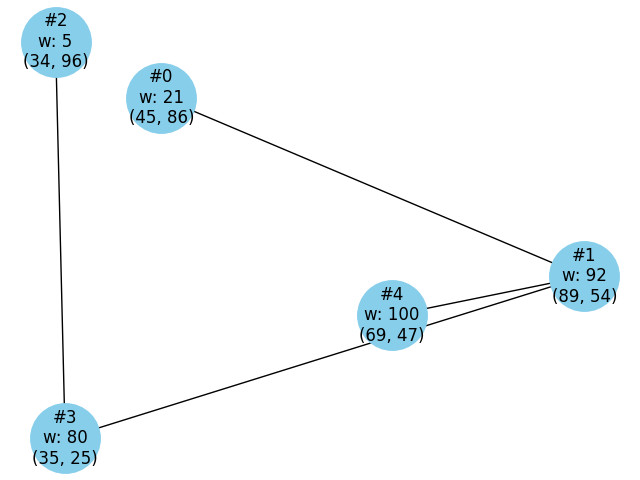
\includegraphics[scale=0.2]{resources/heuristicFail.png}
    \caption{\label{fig:h_fail}Greedy Heuristic failing to output global best}
\end{figure}

The global lightest dominant set of this graph is $[1,2]$ with $w=97.0$

\begin{table}[ht]
    \centering
    \begin{tabular}{|c|c|c|c|}
        \hline
        \textbf{Node} & \textbf{Weight} & \textbf{Neighbors} & \textbf{Weight-Neighbor Ratio} \\
        \hline
        0 & 21 & 1 & 21.0 \\
        \hline
        1 & 92 & 3 & 30.66  \\
        \hline
        2 & 5 & 1 & 5.0  \\
        \hline
        3 & 80 & 2 & 40.0  \\
        \hline
        4 & 100 & 1 & 100.0  \\
        \hline
    \end{tabular}
    \caption{Heuristic's Analysis}
\end{table}

From this table, the order of nodes that the greedy heuristic will chose will be 
$[2,0,1,3,4]$. However, neither $[2]$ nor $[2,0]$, which will be the 2 first
partial constructed solutions from the heuristic, are dominant. Thus, from
continuing the execution the heuristic gets $[2,0,1]$, which is in fact
dominant, and is better than a lot of other dominant sets. Nevertheless, it's
not the lightest dominant set as $w=118$.

\section{Experimental Results}
For replicability of the experiments to remain true, the seed \textit{98374} was used for
every random operation.
\subsection{Number of Operations}

\subsection{Largest problem feasible}

\subsection{Comparison of formal and experimental results} 


\bibliography{...} % use a field named url or \url{} for URLs
% Note: the \bibliographystyle is set automatically

\end{document}
